\documentclass[10pt,letter]{article}
\usepackage{amsmath,amssymb,graphicx,setspace,fullpage,breqn}
\onehalfspacing
\usepackage{fullpage}

\begin{document}
\paragraph*{I.} \textbf{Bijection between order ideals in $\lambda \times [n]$ and increasing tableaux.} 

\subparagraph*{Background.}

We call a nonempty finite subset $\lambda \subset \mathbb{Z}^{d-1}$ a \textit{shape}. Let $e_i$ be the standard basis vector in $\mathbb{R}^{d-1}$. Let $\pi_1(x)$ be the projection onto the $i^{th}$ coordinate.

We say that $\lambda$ is \textit{convex} if whenever $x$ and $x + k \, e_i$ are both contained in $\lambda$, than $x + j e_i \in \lambda$ for $j = 1,...,k-1$.  We say that $\lambda$ is \textit{connected} if for all $x,x' \in \lambda$, there are sequences of coordinates $i_1,...,i_s$ and parities $n_1,...,n_s$ such that $x + \sum_{k=1}^j (-1)^{n_k} e_{i_k} \in \lambda$ for $j = 1,...,s$ and $x + \sum_{k=1}^s e_{i_k} = x'$.  We say that $\lambda$ is \textit{justified} if $\lambda$ lies in the first quadrant and that $\min_{(i,j) \in \lambda} i = \min_{(i,j) \in \lambda} j = 0$. 

Let $\lambda \times [n]$ be the partially ordered set $\lbrace x \times y \in \mathbb{Z}^{d}: x \in \lambda, \ y \in [0,n-1] \rbrace$, where $p \geq q$ if and only if $p -q \in \mathbb{Z}_{\geq 0}^d$. For any poset $P$, we write $J(P)$ to be the collection of order ideals of $P$. 

Let $a_i(\lambda) = \max_{x \in \lambda} \pi_i(x)$ and $a_\lambda = (a_1(\lambda),...,a_n(\lambda)) \in \mathbb{Z}^{d-1}$. Define $\lambda^{\ast} = \lbrace a_\lambda - x: x \in \lambda \rbrace$. It is clear if $\lambda$ is convex/connected/justified, then $\lambda^{\ast}$ is convex/connected/justified. 

For a shape $\mu \subset \mathbb{Z}^{d-1}$, an increasing tableau of height $n$ is a map $T: \mu \rightarrow \lbrace 1,...,n \rbrace$ such that for all $x \in \mu$ and $i = 1,...,{d-1}$, $T(x) > T(x-e_i)$ whenever $x-e_i$ is contained in $\mu$. Let $\text{Inc}^n(\mu)$ be the set of increasing tableaux of height $n$ with base shape $\mu$. 

Any subset of $\mathbb{Z}^d$ is ranked by the function $\text{rk}(x_1,...,x_d) = \sum_{i=1}^d x_i$.

\subparagraph*{The main bijection.}   Define the map $\Phi: J(\lambda \times [n]) \rightarrow \text{Inc}^{\text{max rank}(\lambda)+ n}$ as follows. First define the function $\text{Ht}: \mathbb{Z}_{\geq 0}^{d-1} \times P(\mathbb{Z}_{\geq 0}^d) \rightarrow \mathbb{N}$ so that for $x \in \mathbb{Z}^{d-1}$, $(x,I) \mapsto \max_{(x,y) \in I} y$.  Then define 
\begin{equation*}
\Phi(I) = \bigg( a_{\lambda} - x \mapsto \text{Ht}(x,I) + \text{rk}(a_{\lambda}-x) + 1 \bigg)
\end{equation*}


\paragraph*{II.} \textbf{Equivariance when d = 2.} Following Lemma 4.2, we claim that $\Psi$ intertwines $\text{Pro}_{\text{id},(1,1,-1)}$ and $K$-$\text{Pro}$. Let $\lambda$ be a convex, connected, justified shape in $\mathbb{Z}^2$. Let $a = a_1$ and let $b = a_2$, that is, $(a,b) = a_{\lambda}$.  Take $P \in J(\lambda \times [n])$. 

By Proposition 2.4,  *LIMITS ISSUES*
\begin{equation*}
K\text{-}\text{Pro} = K\text{-}\text{BK}_{a+b+n-1} \circ  ... \circ K\text{-}\text{BK}_1(T)
\end{equation*}
By definition, 
\begin{equation*}
\text{Pro}_{\text{id},(1,1,-1)} = T^{a+b-(a+b+n-1)}_{\text{id},(1,1,-1)} \circ ... \circ T^{a+b}_{\text{id},(1,1,-1)}
\end{equation*}
Therefore it suffices to show 
\begin{equation*}
\Psi(T^{a+b-l}_{\text{id},(1,1,-1)}(P)) = K\text{-}\text{BK}_l(\Psi(P))
\end{equation*}
for all $l$ and all $P \in J(\lambda \times [n])$. 

$T^{a+b-l}_{\text{id},(1,1,-1)}$ is by definition the product of toggles $t_x$ where $x = (i,j,k) \in \lambda \times [n]$ and $\langle x,(1,1,-1) \rangle = i + j - k = a+b - l$. Now if $(i,j,k) \in P$, then $(a-i,b-j)$ is an element of $\lambda^{\ast}$ and is labeled at least $k + \text{rk}(a-i,b-j) + 1= k + (a-i) + (b-j) + 1 = l + 1$. Fix an element $(i,j,k)$ on this hyperplane with $(i,j) \in \lambda$.

\begin{itemize}
\item Say $(i,j,k) \in P$. 
\begin{itemize}
\item On the one hand, if $(i,j,k+1)$ in $P$, then $t_x(P) = P$, since removing $x$ from $P$ would not result in an order ideal. In addition, $K$-$\text{BK}_l$ does not affect entry $(a-i,b-j)$ because $\Psi(P)(a-i,b-j) > l + 1$. 

\item On the other hand, if $(i,j,k+1)$ is not in $P$, then $(a-i,b-j)$ is labeled with $l+1$ so it is affected by $K$-$\text{BK}_l$.  It will only be changed when it is part of a trivial short ribbon, meaning $\Psi(P)(u,v)$ is less than $l$ for all $(u,v) \in \lambda^{\ast}$ covered by $(a-i,b-j)$. The convexity and connectedness assumptions imply that only the elements $(a-i-1,b-j)$ and $(a-i,b-j-1)$ can be covered by $(a-x)$ in $\lambda^{\ast}$.

Say that $(a-i-1,b-j)$ or $(a-i,b-j-1)$ is contained in $\lambda^{\ast}$ and labeled $l$. Then $K$-$\text{BK}_l$ does not change the $(a-i,b-j)$ entry. In addition, either $(i+1,j)$ or  $(i,j+1)$  has height $k$ in $P$. Therefore $P \setminus \lbrace x \rbrace$ is not an order ideal, so $t_x$ does not alter $P$. 

On the other hand, say that neither element is contained in $\lambda^{\ast}$ with label $l$. There are three possibilities:
\begin{itemize}
\item If both positions are part of $\lambda^{\ast}$, and $(a-i-1,b-j) < l$ and $(a-i,b-j-1) < l$, then we are reduced to the case covered in the paper.

\item If one entry, say $(a-i-1,b-j)$ is absent in $\lambda^{\ast}$, and the other has label less than $l$, then $P \setminus \lbrace x \rbrace$ defines an order ideal. For say $(u,v) > (i,j)$ in $\lambda$. By convexity, we must have $v > j$ since $(u,v)$ cannot be contained on the line $\lbrace (i+g,j): g \in \mathbb{Z}_+ \rbrace$, and $u \geq i$. But then $(u,v) \geq (i,j+1)$, and $\Psi(P)(a-i,b-j-1) < l$, so $\text{Ht}(u,v) \leq \text{Ht}(i,j+1) < k$. Since all elements in the column over $(i,j)$ below $(i,j,k)$ are less than $x$, this proves that there is no element in $P$ greater than $x$, so $P \setminus \lbrace x \rbrace$ is an ideal. 


\item Say that both entries are absent in $\lambda^{\ast}$. Then $(i,j)$ is maximal in $\lambda$. For say $(r,s) > (i,j)$ for some $(r,s) \in \lambda$. By connectedness, there is a path from $(i,j)$ to $(r,s)$. By convexity, no element of this path can be contained in the lines $\lbrace (i+g,j): g \in \mathbb{Z}_+ \rbrace$ or  $\lbrace (i,j+g): g \in \mathbb{Z}_+ \rbrace$. Let $(m,n)$ be the first element hit by this path that is greater than $(i,j)$. Such a square must exist because $(r,s) > (i,j)$. Then $(m,n) - (i,j) = (x,0)$ or $(0,x)$ for some $x > 0$. But this point is contained on one of the two excluded lines, a contradiction
\end{itemize}

\end{itemize}

\item Say $(i,j,k) \not \in P$. 
\begin{itemize}
\item If $(i,j,k-1) \not \in P$, then $P \cup \lbrace x \rbrace$ is not an ideal so $t_x$ does not affect $P$. In addition, $\Psi(P)(a-i,b-j) < l$ so $K$-$\text{BK}_l$ does not affect $(a-i,b-j)$.
\item If $(i,j,k-1) \in P$, then $\Psi(P)(a-i,b-j) = l$. $K$-$\text{BK}_l$ will change entry $(a-i,b-j)$ exactly when it is not part of a trivial short ribbon, meaning that all elements that cover it are labeled at least $l + 2$. If either $(a-i+1,b-j)$ or $(a-i,b-j+1)$ is an element of $\lambda^{\ast}$ and is labeled $l+1$, then $(a-i,b-j)$ is unchanged. In addition, this implies that $(i-1,j)$ or $(i,j-1)$ has height $k-1$ respectively, in which case $P \cup \lbrace x \rbrace$ is not an ideal. Otherwise, we have three possibilities as above:
\begin{itemize}
\item If both $(a-i+1,b-j)$ and $(a-i,b-j+1)$ are contained in $\lambda^{\ast}$ and labeled at least $l+2$, then we are reduced to the case from the paper.
\item If one label, say $(a-i+1,b-j)$ is absent from $\lambda^{\ast}$ and the other $(a-i,b-j+1)$ is labeled at least $l+2$, then $P \cup \lbrace x \rbrace$ is an ideal. For say $(u,v) < (i,j)$ in $\lambda$. By convexity, we must have $v < j$ since $(u,v)$ cannot be contained on the line $\lbrace (i-g,j): g \in \mathbb{Z}_+ \rbrace$, and $u \leq i$. But then $(u,v) \leq (i,j-1)$, so $\text{Ht}(u,v) \geq k$, and so $(i,j,k)$. 
\item Finally, if both labels are absent, then $(i,j)$ is minimal as above, so $P \cup \lbrace x \rbrace$ is an ideal.
\end{itemize} 
\end{itemize}
\end{itemize}

\paragraph*{III.} \textbf{Counterexample with $d = 3$}.
\begin{center}
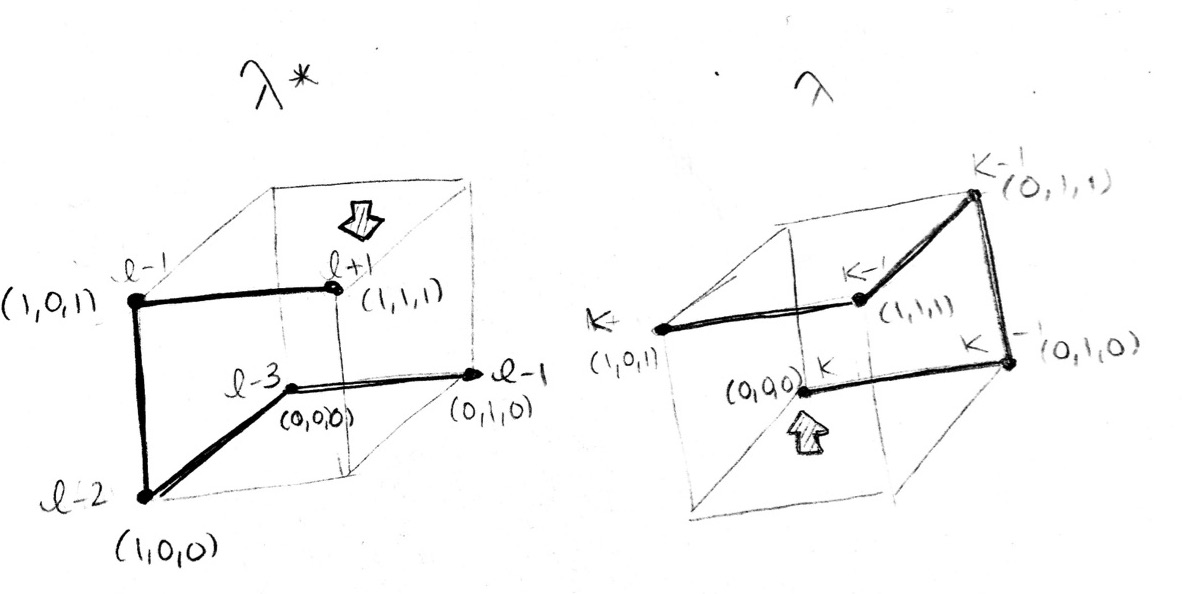
\includegraphics[scale=.4]{counterexample_d3.jpg}
\end{center}
This counterexample shows that $K$-$BK_l$ and $T_x$ will not act in the same way on the tableau of these vertices. For $K$-$\text{BK}_l$ will decrement entry $(1,1,1)$ to $l$, but $T_x$ cannot decrease the height of $(0,0,0)$ because $(1,0,1)$ has height $k$. My guess is that we could successfully replace the convexity condition with the requirement that $\lambda$ be ``twistless,'' defined as the condition that every two elements are connected by a strictly increasing path. 
\end{document}